%
% einleitung.tex -- Beispiel-File für die Einleitung
%
% (c) 2020 Prof Dr Andreas Müller, Hochschule Rapperswil
%
\section{Problem\label{parzyl:section:teil0}}
\rhead{Teil 0}

\subsection{Laplace Gleichung}
Die partielle Differentialgleichung
\begin{equation}
    \Delta f = 0
\end{equation}
ist als Laplace Gleichung bekannt.
Sie ist eine spezielle Form der poisson Gleichung
\begin{equation}
    \Delta f = g
\end{equation}
mit g als beliebige Funktion.
In der Physik hat die Laplace Gleichung in verschieden Gebieten
verwendet, zum Beispiel im Elektromagnetismus.
Das Gaussche Gesetz in den Maxwellgleichungen 
\begin{equation}
     \nabla \cdot E = \frac{\varrho}{\epsilon_0}
\label{parzyl:eq:max1}
\end{equation}
besagt das die Divergenz eines Elektrischen Feldes an einem 
Punkt gleich der Ladung an diesem Punkt ist.
Das elektrische Feld ist hierbei der Gradient des elektrischen
Potentials
\begin{equation}
    \nabla \phi = E.
\end{equation}
Eingesetzt in \eqref{parzyl:eq:max1} resultiert
\begin{equation}
    \nabla \cdot \nabla \phi = \Delta \phi = \frac{\varrho}{\epsilon_0},
\end{equation}
was eine Possion gleichung ist.
An Ladungsfreien Stellen, ist der rechte Teil der Gleichung $0$. 
\subsection{Parabolische Zylinderkoordinaten
\label{parzyl:subsection:finibus}}
Im parabloischen Zylinderkoordinatensystem bilden parabolische Zylinder die Koordinatenflächen.
Die Koordinate $(\sigma, \tau, z)$ sind in kartesischen Koordinaten ausgedrückt mit
\begin{align}
    x & = \sigma \tau \\
    \label{parzyl:coordRelationsa}
    y & = \frac{1}{2}\left(\tau^2 - \sigma^2\right) \\
    z & = z.
    \label{parzyl:coordRelationse}
\end{align}
Wird $\tau$ oder $\sigma$ konstant gesetzt reultieren die Parabeln
\begin{equation}
    y = \frac{1}{2} \left( \frac{x^2}{\sigma^2} - \sigma^2 \right)
\end{equation}
und 
\begin{equation}
    y = \frac{1}{2} \left( -\frac{x^2}{\tau^2} + \tau^2 \right).
\end{equation}

\begin{figure}
    \centering
    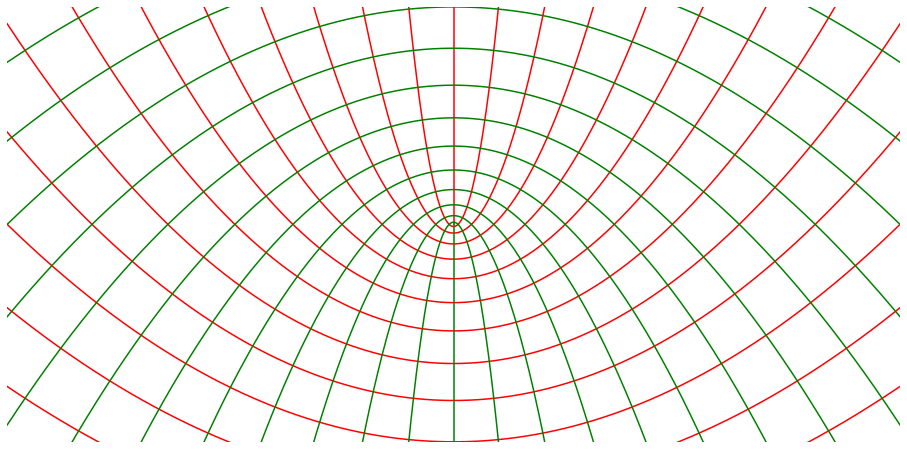
\includegraphics[scale=0.4]{papers/parzyl/img/koordinaten.png}
    \caption{Das parabolische Koordinatensystem. Die roten Parabeln haben ein 
    konstantes $\sigma$ und die grünen ein konstantes $\tau$.}
    \label{parzyl:fig:cordinates}
\end{figure}

Abbildung \ref{parzyl:fig:cordinates} zeigt das Parabolische Koordinatensystem.
Das parabolische Zylinderkoordinatensystem entsteht wenn die Parabeln aus der
Ebene gezogen werden. 

Um in diesem Koordinatensystem integrieren und differenzieren zu 
können braucht es die Skalierungsfaktoren $h_{\tau}$, $h_{\sigma}$ und $h_{z}$.
Der Skalierungsfaktor braucht es, damit die Distanzen zwischen zwei 
Punkten unabhängig vom Koordinatensystem sind.
Wird eine infinitessimal kleine Distanz $ds$ zwischen zwei Punkten betrachtet
kann dies im kartesischen Koordinatensystem mit
\begin{equation}
    \left(ds\right)^2 = \left(dx\right)^2 + \left(dy\right)^2 + 
    \left(dz\right)^2
    \label{parzyl:eq:ds}
\end{equation}
ausgedrückt werden.
Das Skalierungsfaktoren werden so bestimmt, dass
\begin{equation}
    \left(ds\right)^2 = \left(h_{\sigma}d\sigma\right)^2 + 
    \left(h_{\tau}d\tau\right)^2 + \left(h_z dz\right)^2
\label{parzyl:eq:dspara}
\end{equation}
gilt.
Dafür werden $dx$, $dy$, und $dz$ in \eqref{parzyl:eq:ds} mit den Beziehungen
von \eqref{parzyl:coordRelationsa} - \eqref{parzyl:coordRelationse} als
\begin{align}
    dx  &= \frac{\delta x }{\delta \sigma} d\sigma + 
        \frac{\delta x }{\delta \tau} d\tau + 
        \frac{\delta x }{\delta \tilde{z}} d \tilde{z} 
        = \tau d\sigma + \sigma d \tau \\
    dy &= \frac{\delta y }{\delta \sigma} d\sigma + 
        \frac{\delta y }{\delta \tau} d\tau +
        \frac{\delta y }{\delta \tilde{z}} d \tilde{z} 
        = \tau d\tau - \sigma d \sigma \\
    dz &= \frac{\delta \tilde{z} }{\delta \sigma} d\sigma + 
        \frac{\delta \tilde{z} }{\delta \tau} d\tau +
        \frac{\delta \tilde{z} }{\delta \tilde{z}} d \tilde{z} 
        = d \tilde{z} \\
\end{align}
substituiert.
Wird diese gleichung in der Form von \eqref{parzyl:eq:dspara}
geschrieben, resultiert
\begin{equation}
    \left(d s\right)^2 = 
        \left(\sigma^2 + \tau^2\right)\left(d\sigma\right)^2 + 
        \left(\sigma^2 + \tau^2\right)\left(d\tau\right)^2 +
        \left(d \tilde{z}\right)^2.
\end{equation}
Daraus resultieren die Skalierungsfaktoren 
\begin{align}
    h_{\sigma} &= \sqrt{\sigma^2 + \tau^2}\\
    h_{\sigma} &= \sqrt{\sigma^2 + \tau^2}\\
    h_{z} &= 1.
\end{align}
\subsection{Differentialgleichung}
Möchte man eine Differentialgleichung im parabolischen 
Zylinderkoordinatensystem lösen müssen die Skalierungsfaktoren
mitgerechnet werden. 
\dots
